\subsection{WordPress Installation}
After installing Nginx, PHP and MySQL, we can begin with WordPress installation. Please make sure to log in into server-side using PuTTY. Before we can install the WordPress, there are few settings / configurations that have to be done, which includes:
\begin{itemize}
\item Setting up database table and database user
\item Configuring Nginx server
\item Installing additional PHP modules to handle WordPress
\item Generating secret keys
\item Downloading latest stable version of WordPress
\item Configuring WordPress
\end{itemize}

\subsubsection*{Step 1: Creating MySQL Database and User}

First, we need to prepare a database table and user in the installed MySQL. The database table and user will then be used by WordPress to store data and access them.

Start MySQL database by issuing the following command:

\begin{lstlisting}
$ mysql -u root -p
\end{lstlisting}

Enter the password \texttt{d\_XKdEoCwX,4EnO} for the user \texttt{root} when prompted.

Create a new database table \texttt{wordpress} by issuing following command. And don't forget the semicolon at the end of the line.
\begin{lstlisting}
mysql > CREATE DATABASE wordpress DEFAULT CHARACTER SET utf8 COLLATE utf8_unicode_ci;
\end{lstlisting}

Next, create a new user to operate the above created \texttt{wordpress} database. The following command will create a new user \texttt{wordpressuser} with password \texttt{ABcd1234\#}.

\begin{lstlisting}
myql > GRANT ALL ON wordpress.* TO 'wordpressuser'@'localhost' IDENTIFIED BY 'ABcd1234#';
\end{lstlisting}

This will create the new user with given password, as well as granting the user the all accesses to the database \texttt{wordpress}. Finally, flush the privileges so that the MySQL aware of the changes we have made and exit MySQL.

\begin{lstlisting}
mysql > FLUSH PRIVILEGES;
mysql > EXIT;
\end{lstlisting}


\subsubsection*{Step 2: Adjust Nginx's Configuration}
There are two modifications that have to be made to the Nginx web server to handle WordPress correctly:
\begin{enumerate}
\item Instruct server not to log requests for the static files with extensions such as .css, .gif etc.
\item Insert \texttt{index.php} into \texttt{try\_files}
\end{enumerate}

Open the Nginx configuration file using \texttt{sudo} privileges:
\begin{lstlisting}
$ sudo nano /etc/nginx/sites-available/default
\end{lstlisting}

We can request server not to log requests to the static files by issuing command {\tt log\_not\_found off}. It is a best practice not to log requests to static files.

\begin{lstlisting}
server {
	...
	location = /favicon.ico {
		log_not_found off;
		access_log off
	}
	location = /robot.txt {
		log_not_found off;
		access_log off;
		allow all;
	}
	location ~* \.(css|gif|ico|jpeg|jpg|js|png)$ {
		expires max;
		log_not_found off;
	}
	...
}
\end{lstlisting}

For the second task, passing \texttt{index.php} as \texttt{try\_files} is done so that the server will return home page instead of 404 error as a default option. To do this, following line has to put inside \texttt{location /} block.

\begin{lstlisting}
server {
	...
	location / {
		#try_files $uri $uri/ =404;
		try_files $uri $uri/ /index.php$is_args$args;
	}
	...
}
\end{lstlisting}

When these changes have been made, save the configuration file and exit \texttt{nano} editor by pressing \texttt{Ctrl-x}. Check for the syntax errors of the new configurations. If no error is been reported, restart the Nginx.

\begin{lstlisting}
$ sudo nginx -t
$ sudo systemctl reload nginx
\end{lstlisting}

\subsubsection*{Step 3: Installing additional PHP extensions}
PHP preprocessor has been installed and setup with minimal setting in the previous section. Here, additional modules or extensions will be installed, which is required by WordPress. Use to following command to install the required additional extensions:

\begin{lstlisting}
$ sudo apt-get update
$ sudo apt-get install php-curl php-gd php-mbstring php-mcrypt php-xml php-xmlrpc
\end{lstlisting}

After finish installing the extensions, restart the \texttt{php-fpm} process.
\begin{lstlisting}
$ sudo systemctl restart php7.0-fpm
\end{lstlisting}

\subsubsection*{Step 4: Generating secret keys}
Secret keys have to be generated to provide security for the WordPress. The secret keys are provided by WordPress through their secure key generator. To get secret keys from WordPress key generator, issue the following command on the terminal:

\begin{lstlisting}
$ curl -s https://api.wordpress.org/secret-key/1.1/salt
\end{lstlisting}

Or another workaround is to use the web browser. Enter the URL \texttt{https://api.wordpress.org/secret-key/1.1/salt} and press enter. Save the generated secret keys, which must be used in the next step.


\subsubsection*{Step 5: Downloading WordPress}
Download the latest version of stable WordPress from https://wordpress.org website. After downloading, extract the downloaded content.

\begin{lstlisting}
$ cd /tmp
$ curl -o https://wordpress.org/latest.tar.gz
$ tar xzvf latest.tar.gz
\end{lstlisting}

By default, WordPress has provided a sample copy of the WordPress configuration file. This file can be found under directory and file name \texttt{tmp/wordpress/wp-config-sample.php}.

Copy the provided configuration file to used in our website. And Create a new directory \texttt{upgrade}, so that WordPress can upgrade its software in the future without any permission issue.
\begin{lstlisting}
$ cp /tmp/wordpress/wp-config-sample.php /tmp/wordpress/wp-config.php
$ mkdir /tmp/wordpress/wp-content/upgrade
\end{lstlisting}

Finally, copy the contents into root server directory. This are the contents used by the Nginx web server to serve when request is made to the website.
\begin{lstlisting}
$ sudo cp -a /tmp/wordpress/. /var/www/html
\end{lstlisting}

\subsubsection*{Step 6: Configuring WordPress}
Open the WordPress configuration file:
\begin{lstlisting}
$ nano /var/www/html/wp-config.php
\end{lstlisting}

In the file, find the 'secret key' section, which appears as follow and paste the generated secret keys from Step 4.
\begin{lstlisting}
...
define('AUTH_KEY', 'put your unique phrase here');
define('SECURE_AUTH_KEY', 'put your unique phrase here');
define('LOGGED_IN_KEY', 'put your unique phrase here');
define('NONCE_KEY', 'put your unique phrase here');
define('AUTH_SALT', 'put your unique phrase here');
define('SECURE_AUTH_SALT', 'put your unique phrase here');
define('LOGGED_IN_SALT', 'put your unique phrase here');
define('NONCE_SALT', 'put your unique phrase here');
...
\end{lstlisting}


After pasting the generated secret keys, the MySQL database credentials have to be given. These credentials have been created in the Step 1.
\begin{lstlisting}
...
define('DB_NAME', 'wordpress');

/** MySQL database username */
define('DB_USER', 'wordpressuser');

/** MySQL database password */
define('DB_PASSWORD', 'ABcd1234#');
\end{lstlisting}

Lastly, we need to give permission to Nginx web server to write where it needs to. Otherwise, WordPress will be asking FTP credentials when any actions need to be performed. This can be done through following setting:
\begin{lstlisting}
define('FS_METHOD', 'direct');
\end{lstlisting}

Save the \texttt{wp-config.php} file and exit the nano editor.

\subsubsection*{Step 7: Complete WordPress Installation}
We need to complete the WordPress installation now through the web browser. Open the web browser and enter the URL \texttt{192.168.0.20}. First, we need to select the language.

\begin{figure}[h]
\caption{WordPress language selection}
\centering
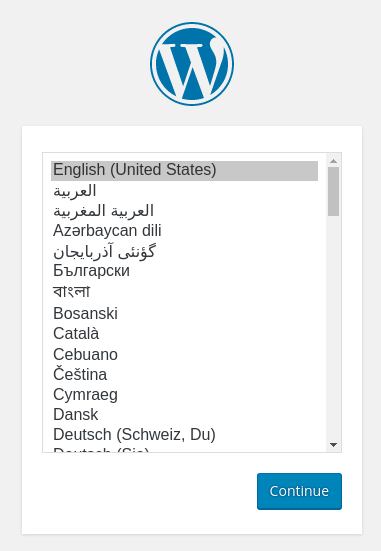
\includegraphics[height=5cm,keepaspectratio]{language-selection.png}
\end{figure}

After that, we need to provide a few information on the main setup page such as \emph{Site Title}, \emph{Username}, \emph{Password} and \emph{Email}.

\begin{figure}[h]
\caption{Main WordPress setup page}
\centering
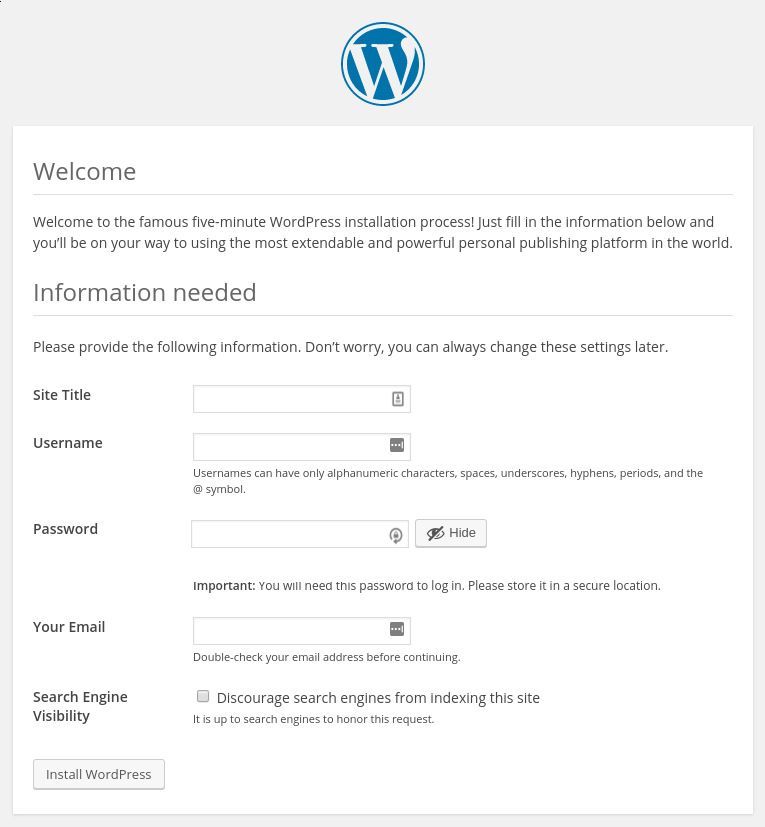
\includegraphics[height=6cm,keepaspectratio]{main-wp-setup.png}
\end{figure}

These are information given on the page shown above:
\begin{itemize}
\item Site Title: Smart Home Lab
\item Username: ashiqmoh
\item Password: oSm0cCCAguIMsalrZd(\#2i5(
\item Email: ashiqmoh@192.168.0.20
\end{itemize}

The installation can be completed by clicking 'Install WordPress' button. Upon installation, the administration side of the website can be accessed by entering following URL:
\begin{lstlisting}
http://192.168.0.20/wp-admin
- or -
http://web.smarthome.hs-furtwangen.de/wp-admin
\end{lstlisting}

Provide the username and password stated above and login. The administration side of the website appears as shown in the figure below.

\begin{figure}[h]
\caption{Administation page of WordPress}
\centering
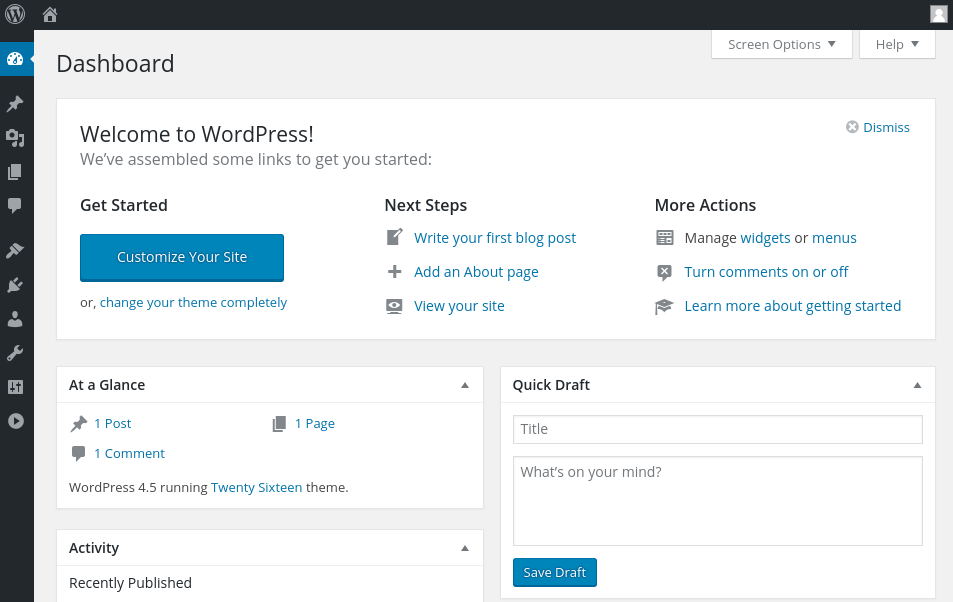
\includegraphics[height=7cm,keepaspectratio]{wp-admin-page.png}
\end{figure}